\documentclass[../main.tex]{subfiles}




\begin{document}




\subfile{anells/anells.tex}
\subfile{moduls/moduls.tex}
\subfile{anells i moduls de fraccions/fraccions.tex}
\subfile{anells i moduls noetherians/noetherians.tex}
\subfile{anells de Dedekind/dedekind.tex}


\appendix
\subfile{appendix/appendix.tex}
\newpage
\chapter{Mòduls projectius i injectius}
A continuació adjuntaré d'una forma molt cutre els apunts que va proporcionar-nos Santiago Zarzuela, que tracten els mòduls projectius i injectius amb més detall. No cal tot per fer el seguiment del curs, però algunes coses són importants i rellevants en altres camps de les matemàtiques (e.g., teoria de representacions de grups). 

Comença a la següent pàgina.
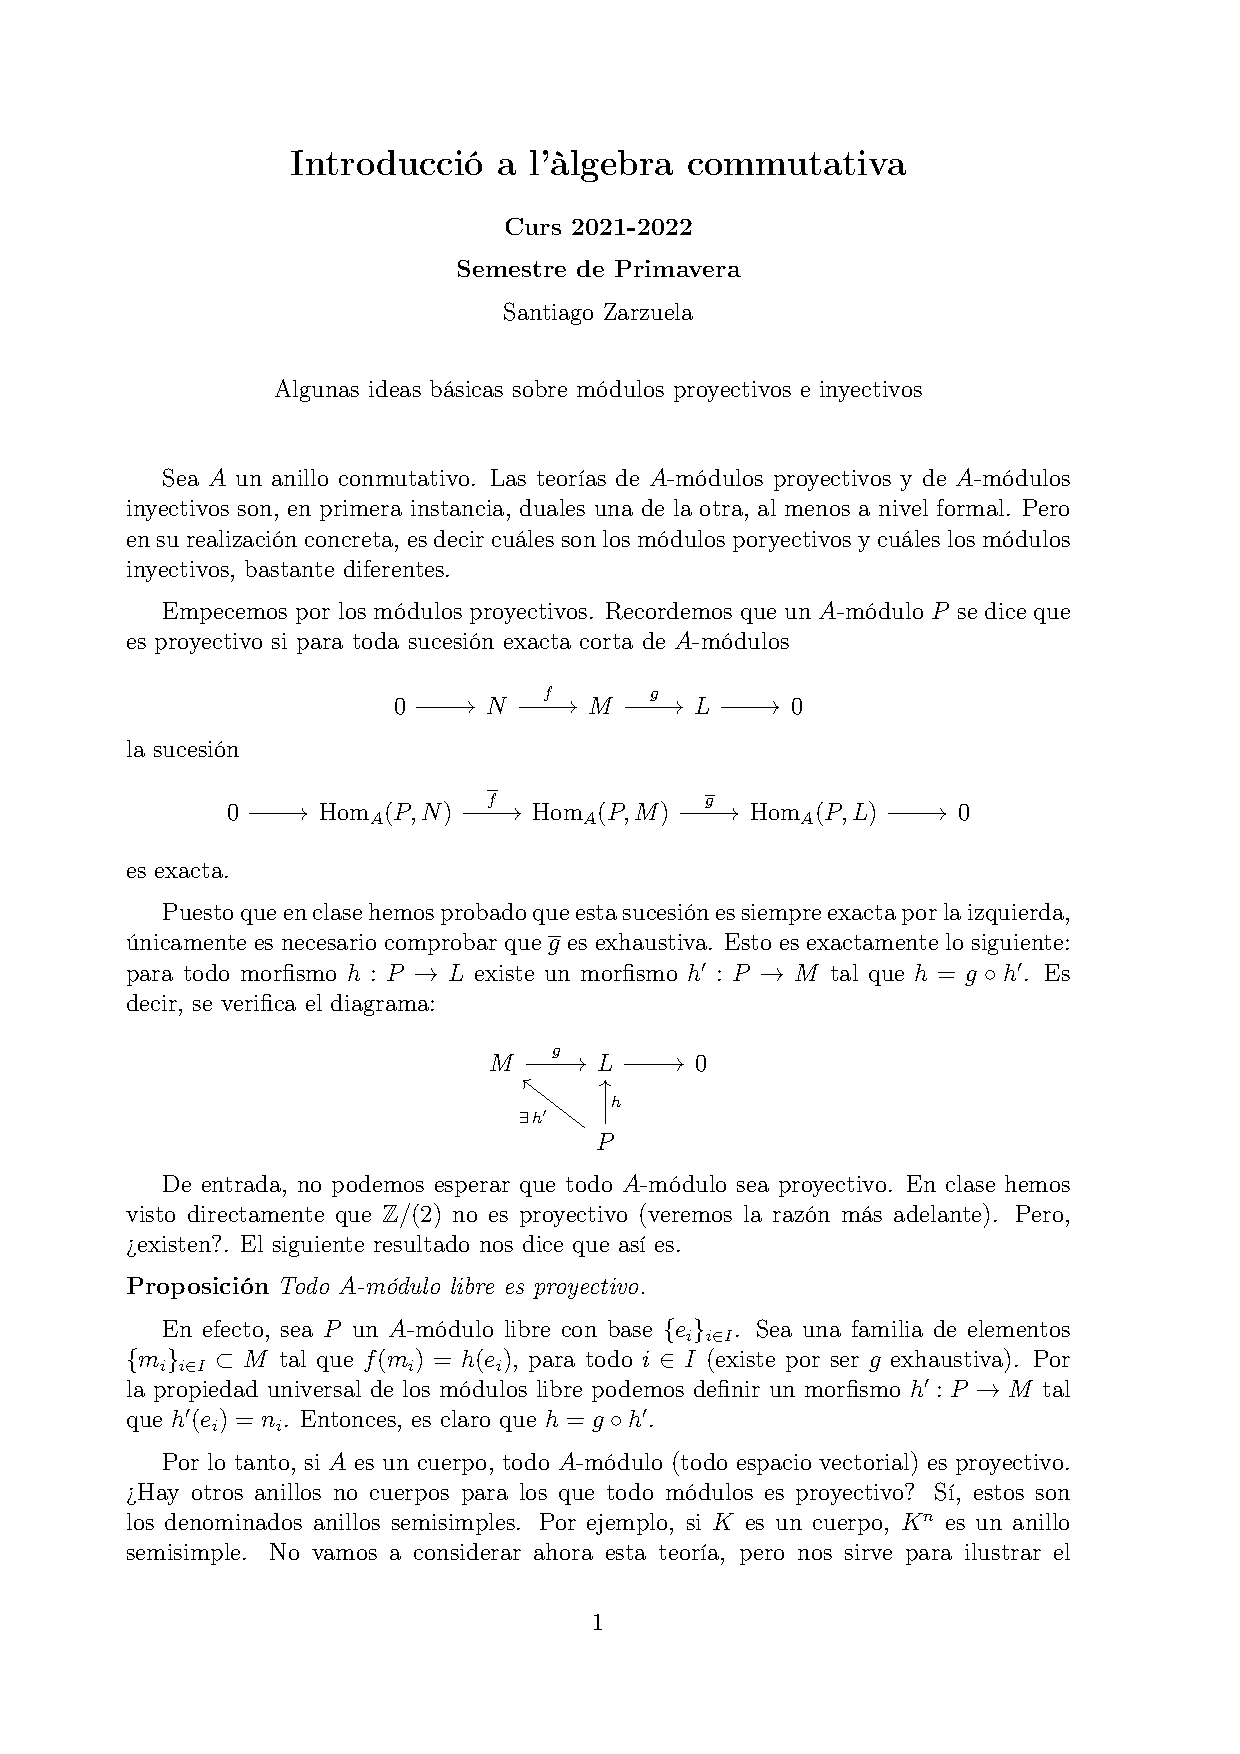
\includepdf[pages=-,pagecommand={},width=\textwidth]{proyectivos.pdf} % para insertar pdf











\end{document}